\section{Costs}

The presence of the breakwater must lead to a reduction in mooring costs, because wave energy will be dissipated or reflected such that the drift forces on the floating island are reduced. Therefore, a cost function is introduced in section \ref{sec: mooring costs} which quantifies the costs of the mooring system as function of the drift forces.  The inclusion of a breakwater only makes sense if the costs of the breakwater are lower than the cost reduction in mooring costs. So, a cost function for the expenses on the breakwater are presented in section \ref{sec: breakwater costs}.


%Also, the floating island will experience less motions when the right breakwater is placed, which increases the workability on the island modules and connector costs will be less. Therefore, a cost function which quantifies these effects as function of the breakwaters transmitted wave height will be introduced in section \ref{sec: work and connector costs}.


\subsection{Mooring costs}
\label{sec: mooring costs}

% An estimation was made for the mooring costs by using the the public deliverable D1.3 from Space@Sea. In this document is referred to a document where the exact composition of the mooring costs can be found. Unfortunately, this document is confidential. Thereby, an estimation was made by the following calculation. D1.3 gave a total of \texteuro 20 M for the total mooring system of the floating island, schematized by the following picture

% -estimation mooring costs Space@Sea\\
% -Delivarable 1.3: total mooring system costs \texteuro 20 M\\
% -So, one row of breakwaters would cost roughly \texteuro 20/9 M.
% -That mean wave drift force scales linearly with the amount of euros 

The future mooring costs of the island when a breakwater is connected to its wave-ward side is computed in this section. In Space@Sea, an extensive research was done on the design of the mooring system of the North Sea case, based on the wind, wave and current conditions on that location. Therefore, this mooring system design with its costs are taken as benchmark for the estimation of the reduction in mooring costs. In section \ref{subsec: mooring design S@S} it is investigated how the mooring design was constructed in order to make an as accurate as possible cost function for the future mooring costs of what the mooring system would cost when a breakwater is present. This cost function is elaborated in section \ref{subsec: reduction mooring costs function}.


% \subsection{Mooring design Space@Sea}
% \label{subsec: mooring design S@S}
A cost function of the mooring system as function of the drift forces is made by using the total mooring costs of Case 2 of the Space@Sea project, where the island shown in figure \ref{fig: mooring layout S@S} will cost \texteuro 20 M. Since a two-dimensional breakwater is studied, this setup is simplified to a single row of nine island modules. It is assumed this will cost $\frac{1}{9}$th of the total mooring costs, which is approximately \texteuro 2.22 M. Dividing this through 45 (=module width) leads to \texteuro 49.382,71 per unit width of floating island. This design is made based on a peak mean wave drift force of 120.7 MN, which is caused by the wind, current and the waves. In the following sections the magnitude of contribution of each phenomena is investigated. 
\begin{figure}[H]
    \centering
    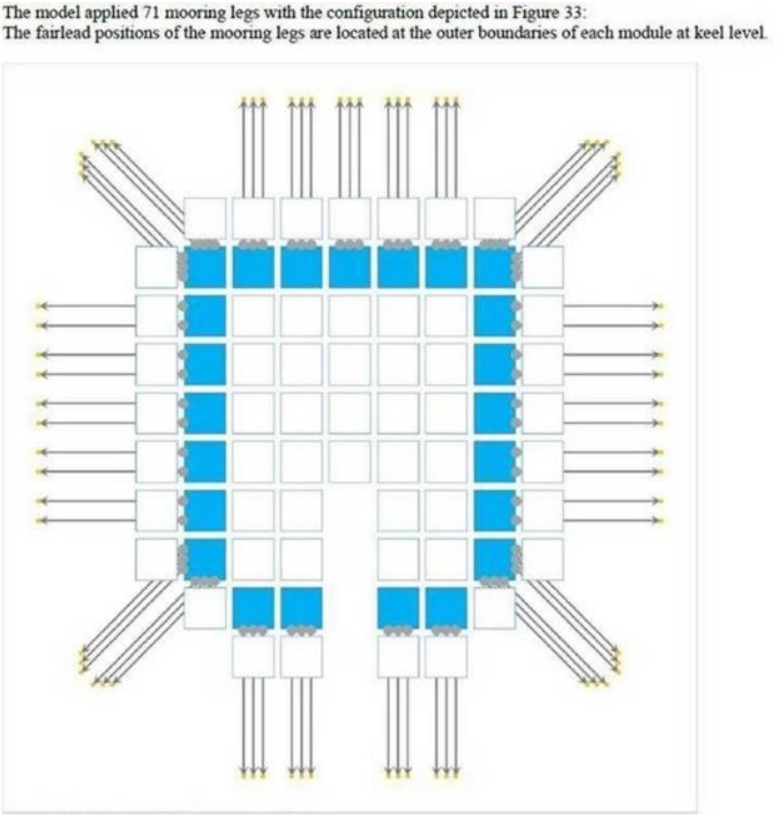
\includegraphics[width=0.5\linewidth]{figures/Costs/mooring_layout.PNG}
    \caption{Mooring layout Space@Sea (ref to source, D1.3)}
    \label{fig: mooring layout S@S}
\end{figure}



\subsubsection{Wind Load}
The contributions from wind loads are applied using the following \acrfull{OCIMF} convention \cite{D3.3space@sea}:
\begin{equation}
    F_{x,w} = \frac{1}{2} \cdot \rho_a \cdot C_{x,w} \cdot V_w^2 \cdot A_T
\end{equation}
In the design of the mooring system of Space@Sea the following parameters are used:
\begin{itemize}
    \item Air density $\rho_a$ = 1.225 $kg/m^3$
    \item Coefficient $C_{x,w}$ = 1
    \item Wind velocity $V_w$ = 29.5 $m/s$
    \item Transverse surface area above water $A_T$ = 225 $m^2$
\end{itemize}
This results in a design wind load per unit width of $F_{x,w}~\approx$ 239.86 kN. Dividing this through the floater width gives a wind design load of $F_{x,w}~\approx$ 5.33 kN/m

\subsubsection{Current Load}
The current load used for the design of the mooring system of Space@Sea is calculated according the \acrshort{OCIMF} convention as well:
\begin{equation}
    F_{x,w} = \frac{1}{2} \cdot \rho_w \cdot C_{x,c} \cdot V_c^2 \cdot W \cdot T
\end{equation}
where the following parameters are used:
\begin{itemize}
    \item Sea water density $\rho_w$ = 1000 $kg/m^3$
    \item Coefficient $C_{x,c}$ = 1
    \item Current velocity $V_c$ = 2.0 $m/s$
    \item Module width $W$ = 45 $m$
    \item Module depth $T$ = 6 $m$
\end{itemize}
This results in a current design load of $F_{x,c}~ = $ 540.00 kN. Which results in a current design load per unit width of $F_{x,c}~ = $ 12.00 kN/m\\
\\
\subsubsection{Wave load}
The peak mean wave drift force used in the design of the mooring system of the total island (see figure \ref{fig: mooring layout S@S}) is 120.7 MN \cite{D3.3space@sea}. Per unit width is this 297.93 kN/m. From which 12.00 kN/m is due to the current and 5.33 kN/m is due to the wind. So, contribution to the mean wave drift force delivered by the waves is 280.60 kN/m, which is 94 \% of the total mean wave drift force.\\
\\
This big proportion of the contribution of the waves to the maximum mean wave drift on the island emphasises the potential added value the breakwater can have, but does not mean we can neglect the other contributions by the wind and the current. Six percent may seem negligible, but when a breakwater succeeds in attenuating the waves substantially, this ratios will be very different. Especially since the height of the mean wave drift force on the floating island scales to the height of the waves interacting with the island squared. \\


\subsection{Reduction mooring costs due to presence of breakwater}
\label{subsec: reduction mooring costs function}
This rest of the section explains how the reduction of mean wave drift forces on the floating island quantify in a reduction of mooring costs. In \cite{D3.3space@sea} is stated that the mooring system is designed for a peak mean wave drift force of 120.7 MN. To convert this to a single row of modules again, $\frac{1}{9}$th of that force will be 13.4 MN and dividing this through 45 leads to 0.30 MN of design drift force per unit with of floating island. The mean wave drift force scales to the height of the incoming wave squared. Together with the assumption that the cost of the mooring system scales linearly to the mean wave drift force acting on the island, the reduction on mooring costs is derived as follows.


\begin{equation}
\begin{array}{lll}
    H^2 & \propto F\\
    \\
    F & \propto \\
    \\
    \texteuro_{mooring} & \propto H^2
\end{array}
\end{equation}


% \begin{equation}
% \begin{array}{lll}
%     \text{\texteuro}_{new~mooring~island} = \text{\texteuro}_{old~mooring~island} \cdot \frac{H_{t,breakwater}}{H_{i,breakwater}}^2\\
%     \\
%     \text{\texteuro}_{mooring~breakwater} = \text{\texteuro}_{old~mooring~island} \cdot \frac{\bar{F_{d, breakwater}}}{F_{d, island}}\\
%     \\
%     \text{\texteuro}_{total~mooring} = \text{\texteuro}_{new~mooring~island} + \text{\texteuro}_{mooring~breakwater}

% \end{array}
% \end{equation}

Leads to
\begin{equation}
    \text{\texteuro}_{new~mooring~island} =  \text{\texteuro}_{old~mooring~island} \cdot (0.06+ 0.94\cdot \frac{H_{t,breakwater}}{H_{i,breakwater}}^2)
    \label{eq: new mooring island costs}
\end{equation}
\begin{equation}
    \text{\texteuro}_{mooring~breakwater} = \text{\texteuro}_{old~mooring~island} \cdot \frac{\bar{F_{d, breakwater}}}{F_{d, island}}\\
    \label{eq: mooring costs breakwater}
\end{equation}
\begin{equation}
    \text{\texteuro}_{total~mooring} = \text{\texteuro}_{new~mooring~island} + \text{\texteuro}_{mooring~breakwater}
    \label{eq: total mooring costs}
\end{equation}
\begin{equation}
    \texteuro_{reduction~mooring~costs} = \texteuro_{old mooring island}- \texteuro_{total mooring}
    \label{eq: reduction mooring costs}
\end{equation}
All quantities are per unit width. In formula \ref{eq: new mooring island costs}, the design mooring costs of \texteuro 49.382,71 is used for $\text{\texteuro}_{old~mooring~island}$, the ratio between the transmitted wave height and the incident wave height is used with the calculation of $\text{\texteuro}_{new~mooring~island}$, which is the new height off the mooring costs of the floating island due to the wave attenuation of the breakwater. The transmission coefficient ($H_t/H_i$) has only an influence on 94\% of the new mooring costs. In other words, when 100\% of the wave is attenuated by the breakwater ($H_t/H_i$ = 1), no drift forces are present due to the waves, but the current and wind can still give a load on the mooring lines and 6\% of the old mooring costs will still be present.
Formula \ref{eq: mooring costs breakwater} defines the costs of the mooring system of the breakwater itself, using again the design costs of the floating island of Space@Sea times the ratio of the mean wave drift force on the breakwater and the mean wave drift force where the design mean wave drift force of the Space@Sea island. Note that this quantity can by negative, when a negative mean wave drift force on the breakwater is experienced.
The outcome of the two latter formulas lead to the total costs of the mooring system: $\text{\texteuro}_{total~mooring}$ in formula \ref{eq: total mooring costs} and this is used to calculate the eventual reduction in mooring costs due tot the presence of the breakwater $\texteuro_{reduction~mooring~costs}$ in \ref{eq: reduction mooring costs}.




% In figure \ref{fig: strip modules} a this single strip of island modules is shown schematically. The drift force used in the determination of the required mooring system is estimated by calculating the mean wave drift force of this system when waves are coming from the left, because from this direction the highest drift loads will occur. The wave characteristics of the highest waves possible at the location on the North Sea (\textbf{include HKN ref}) are used in the calculation: H = 9 meters and T$_p$ = 10.4 seconds. The drift force on each individual module is estimated using the Macagno formula and the formula of the mean wave drift force on a box-type breakwater derived by \cite{longuethiggins1977}. Where the Macagno formula (equation \ref{eq: macagno1953}) derives the transmitted and reflected wave height of each island module, which are used as input in the calculation of the mean wave drift force in equation \ref{eq: longuethiggins force}. So, the mean wave drift force of each individual module is calculated, where its incident wave height on a module is the transmitted wave height of the previous module. The results of this calculation are shown in table \ref{tab: results table mean wave drift force }


% \begin{equation}
%     K_{\mathrm{t}}=\frac{1}{\sqrt{1+\left[\frac{k W_{\mathrm{f}} \sinh (k h)}{2 \cosh \left(k h-k T_{\mathrm{f}}\right)}\right]^{2}}}
%     \label{eq: macagno1953}
% \end{equation}
% \begin{equation}
%     \Bar{F} = \frac{1}{16}\rho g (H_i^2 + H_r^2 - H_t^2)(1 + \frac{2kh}{sinh(2kh)})
%     \label{eq: longuethiggins force}
% \end{equation}

% \begin{figure}[H]
%     \centering
%     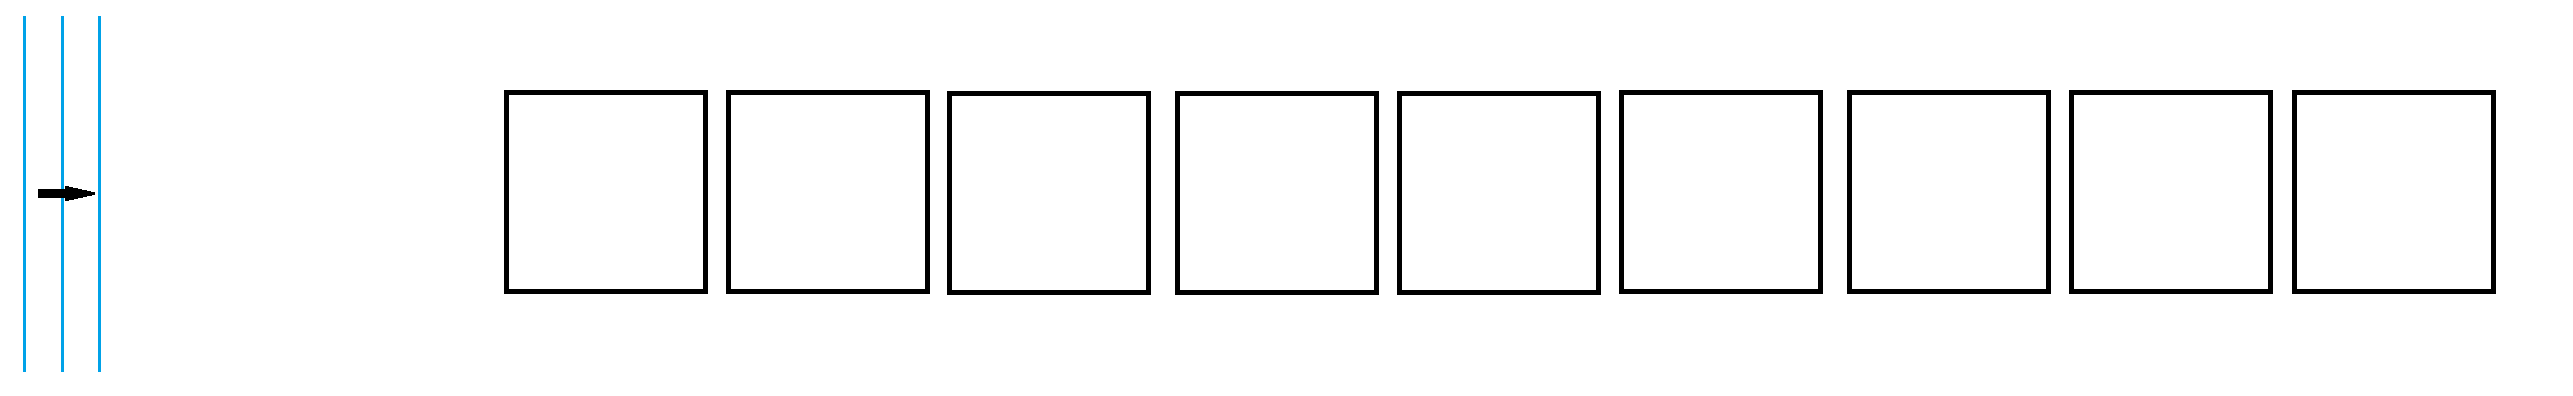
\includegraphics[width=0.8\linewidth]{figures/Costs/mooring_layout_singlerow_without_breakwater.png}
%     \caption{Strip of island modules}
%     \label{fig: strip modules}
% \end{figure}

% % Please add the following required packages to your document preamble:
% % \usepackage{booktabs}
% \begin{table}[H]
% \centering
% \begin{tabular}{@{}lllll@{}}
% \toprule
% Island module & H$_i$ {[}m{]} & H$_r$ {[}m{]} & H$_t$ {[}m{]} & $\Bar{F}$ {[}N{]} \\ \midrule
% 1             & 9.00          & 6.64          & 6.08          & 8.33E4            \\
% 2             & 6.08          & 4.48          & 4.10          & 3.80E4            \\
% 3             & 4.10          & 3.03          & 2.77          & 1.73E4            \\
% 4             & 2.77          & 2.04          & 1.87          & 7.91E3            \\
% 5             & 1.87          & 1.38          & 1.26          & 3.61E3            \\
% 6             & 1.26          & 0.93          & 0.85          & 1.65E3            \\
% 7             & 0.85          & 0.63          & 0.58          & 7.50E2            \\
% 8             & 0.58          & 0.43          & 0.39          & 3.42E2            \\
% 9             & 0.39          & 0.29          & 0.26          & 1.56E2            \\ \midrule
%               &               &               & Total:        & 1.23E5            \\ \bottomrule
% \end{tabular}
% \caption{Results estimation mean wave drift force }
% \label{tab: results table mean wave drift force }
% \end{table}


% \subsection{Mean wave drift force with breakwater}

% From the output of ComFLOW, a transmitted wave height and a mean wave drift force will be determined for each configuration of breakwater. To calculate the mean wave drift force of the system shown in figure \ref{fig:strip modules with breakwater}, where the breakwater is displayed in red, the same calculation is done as described in the previous section. Except the incident wave height of the first island module will be the transmitted wave height determined by ComFLOW. And the drift force acting on the breakwater will be summed to the result to obtain the total mean wave drift force. 


% \begin{figure}[H]
%     \centering
%     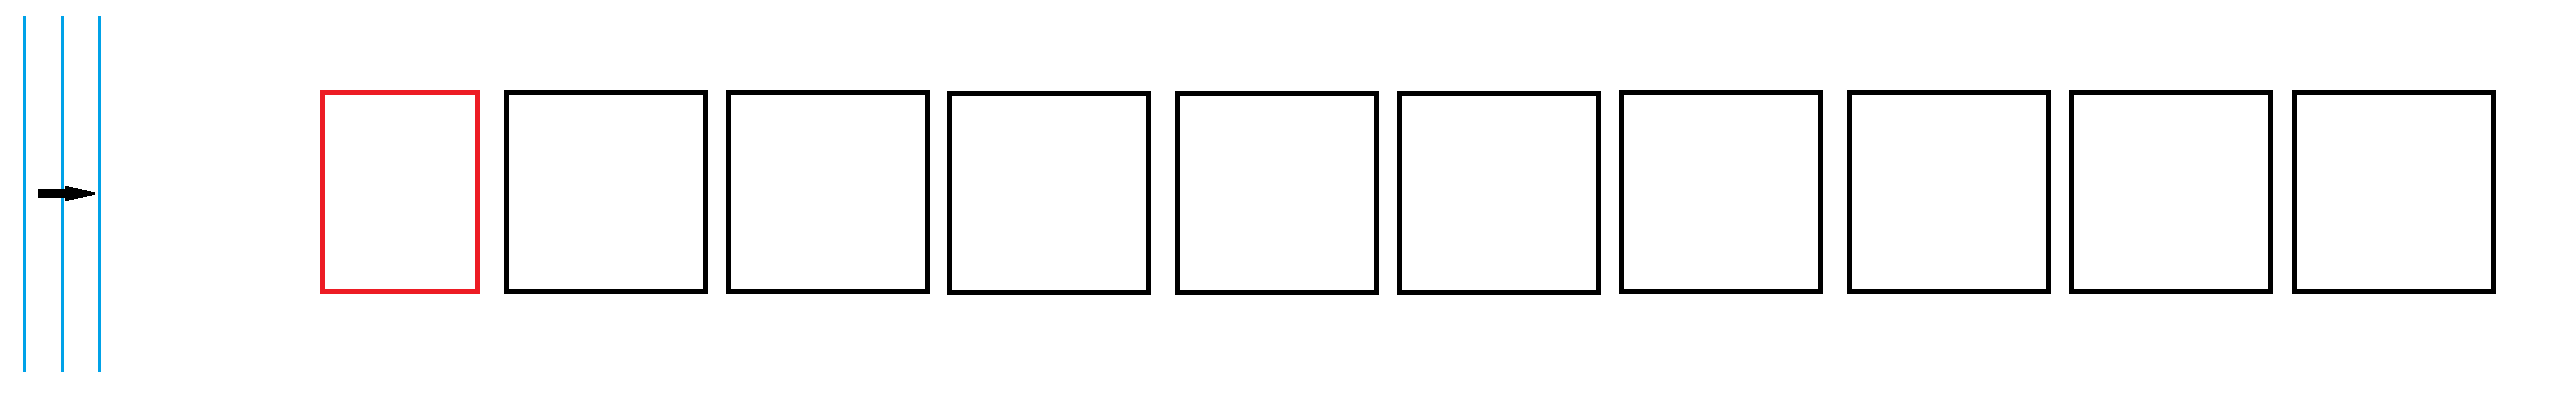
\includegraphics[width=0.8\linewidth]{figures/Costs/mooring_layout_singlerow_with_breakwater.png}
%     \caption{Strip of island modules with breakwater}
%     \label{fig:strip modules with breakwater}
% \end{figure}

% The total mean wave drift force of the system (nine island modules and the breakwater) will be a certain fraction of the mean wave drift force of the system without breakwater. With the assumption that the costs of the mooring system will scale linearly with the mean wave drift force, this fraction can be used to determine the reduction in mooring costs due tot the presence of the breakwater. This can be described by the following equation:

% \begin{equation}
%     \texteuro_{total}M = \frac{\Bar{F}_{with breakwater}}{\Bar{F}_{without breakwater}} \cdot \texteuro 2.22M
% \end{equation}

% \subsubsection{Drift force due to current}
% \begin{equation}
% F_{X, C}=\frac{1}{2} \cdot \rho_{C} \cdot C_{X, C} \cdot V_{C}{ }^{2} \cdot L_{B P} \cdot T
% \end{equation}

% Note: is of little influence is said in \cite{S@S_demonstationatwavetank}.
% Assumed to work only on first module!


% \subsubsection{Drift force due to wind}
% \begin{equation}
% F_{X, W}=\frac{1}{2} \cdot \rho \cdot C_{x, w} \cdot V_{w}{ }^{2} \cdot A_{T}
% \end{equation}
% Assumed to work only on first module!

% \subsubsection{Drift force on modules due to waves}
% uitleg script: (onderstaand is verouderd)
% To determine what the complete drift force of one row of 9 island modules is, during the most extreme wave conditions on the North Sea: H=9m and T = 10.4s, equation \ref{eq: total drift force} is used. Therefore, the incident, reflected and transmitted wave height on each module is determined by the Macagno formula (equation \ref{eq: macagno1953}). This resulted in a total force of: 153127.623164916 Newton. So, the amount of euros on the mooring system per Newton drift force: \texteuro $\frac{20}{9}$M$/ F_{total} \approx$ 14.51  \texteuro/N.\\
% \\

% The drift force linearly scales with the part of the drift force on modules due to waves, while the wind and current part stays constant.\\
% \\
% Only first component of QTF (look at offshore hydromechanics for explanation)




\section{Breakwater costs}
\label{sec: breakwater costs}
To determine the costs of the breakwater the mass of the breakwater is used. It is assumed the construction is made of steel and concrete. This material is relatively cheap and makes a good combination because concrete is resistant to compression and steel to tension, while they have roughly the same thermal expansion coefficient.\\
\\
In deliverable 1.2 of the Space@Sea project (\cite{Adam2017D1.2S@S}), a business case is done for a energy hub which is aiming at providing accommodation and working space for offshore workers. An extensive research is done for what the costs would be of such floating structures. Here, it is estimated the steel and concrete carcass of the structure would have a mass of 9300 ton and would cost \texteuro 9.611.077. From this 9300 ton, 5407 ton (58\%) ton would be steel and 3893 ton (42\%) concrete. The price of concrete is roughly  775 \texteuro/ton and the price of steel varies from 2000 \texteuro/ton to 4000 \texteuro/ton, depending on the labour needed to manufacture the construction. These prices and mass ratios are used for the estimation of the \acrshort{capex} costs of the breakwater.\\
\\
So, the height of the steel price is different for each breakwater. A box-type structure can be made for 2000 \texteuro/ton and a skew floating beach can be made for 4000 \texteuro/ton. This variation is made into a function the following way; the rectangular parts of the breakwater are made for 2000 \texteuro/ton and the variable part varies between 2000 and 4000 \texteuro/ton (red part in figure \ref{fig: steel price breakwater}), depending on the angle $\alpha$ with the following formula:
\begin{equation}
    for ~ 0\textdegree ~\alpha<45 \textdegree~:~ \texteuro_{steel} = 4 - \frac{2}{45} \cdot alpha
\end{equation}
\begin{equation}
        for ~ 45\textdegree~<\alpha<90\textdegree ~:~\texteuro_{steel} =\frac{2}{45} \cdot alpha
\end{equation}
\begin{figure}
    \centering
    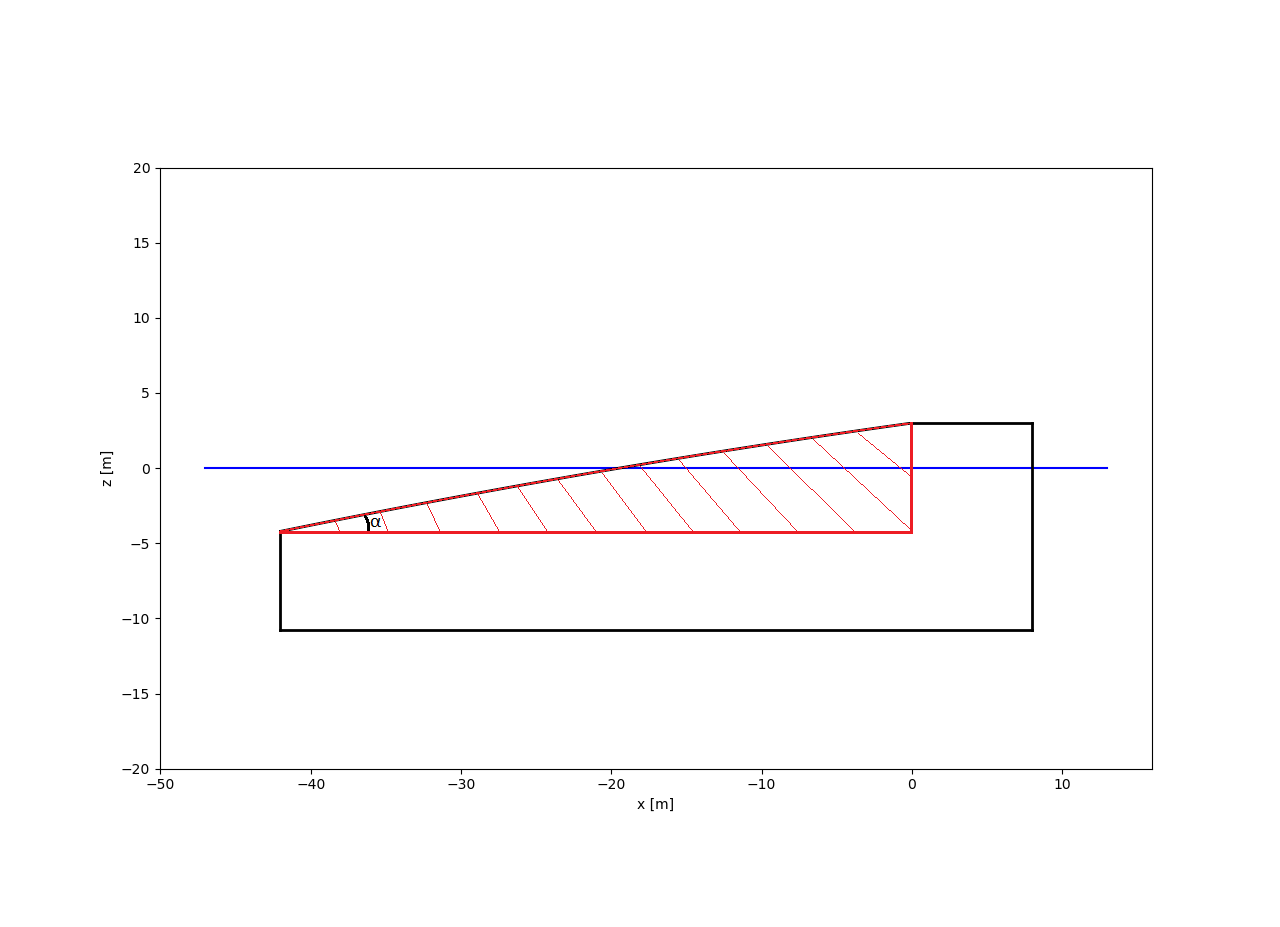
\includegraphics[width=0.9\linewidth]{figures/Costs/breakwater_1.png}
    \caption{Caption}
    \label{fig: steel price breakwater}
\end{figure}
This way the price reaches its maximum (4000 \texteuro/ton) when a very skew slope is desired and its minimum (2000 \texteuro/ton) when $\alpha=45 \textdegree$. \\
\\




Of course, the market price of concrete can vary in time as well, but the amount of labour put into the manufacturing of the concrete is hardly affected by the breakwaters shape. Because it is poured in fluidly after the framework is created and takes in the proper shape by itself. Thereby, the price of the concrete is assumed to be constant with a price of 775 \texteuro/ton for the breakwaters. \\
\\

\section{Results}


\begin{figure*}[h]
    \centering
    \begin{subfigure}[b]{0.475\textwidth}
        \centering
        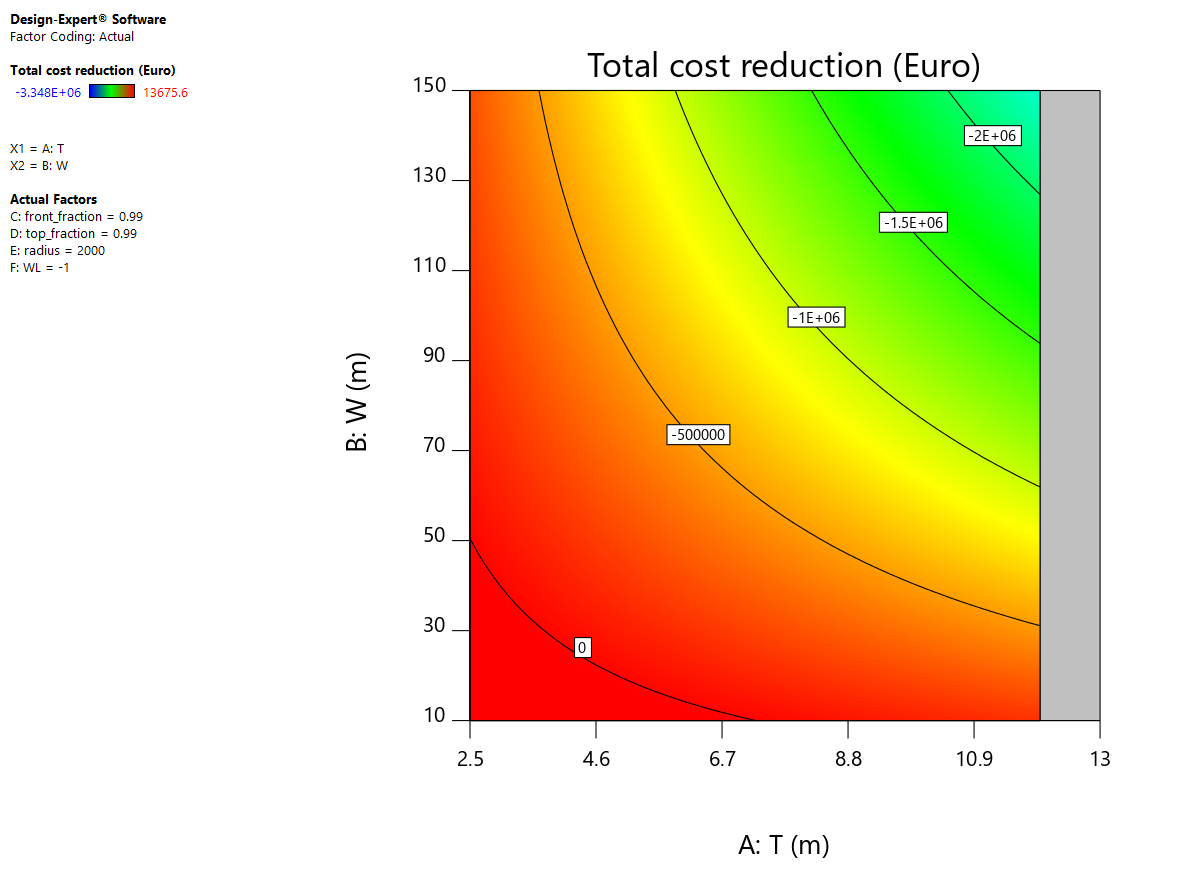
\includegraphics[width=\textwidth]{figures/ComFLOW/Results DI1/costs/W_T_Costs_total_reduction_box_png.png}
        \caption[]%
        {{\small }}    
        \label{fig: opt }
    \end{subfigure}
    \hfill
    \begin{subfigure}[b]{0.475\textwidth}  
        \centering 
        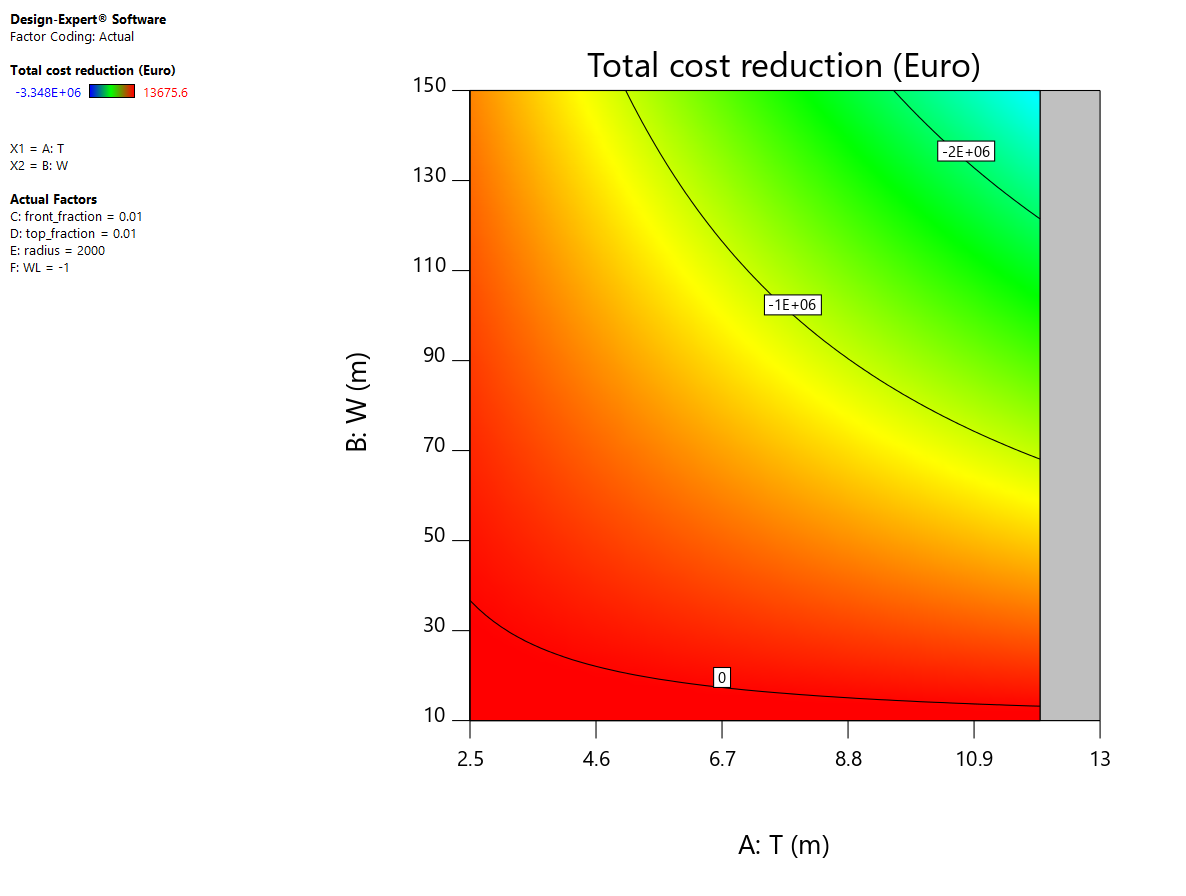
\includegraphics[width=\textwidth]{figures/ComFLOW/Results DI1/costs/W_T_Costs_total_reduction_wedge_png.png}
        \caption[]%
        {{\small }}    
        \label{fig: opt }
    \end{subfigure}
    \caption{}
    \label{fig: }
\end{figure*}

\begin{figure*}[h]
    \centering
    \begin{subfigure}[b]{0.475\textwidth}   
        \centering 
        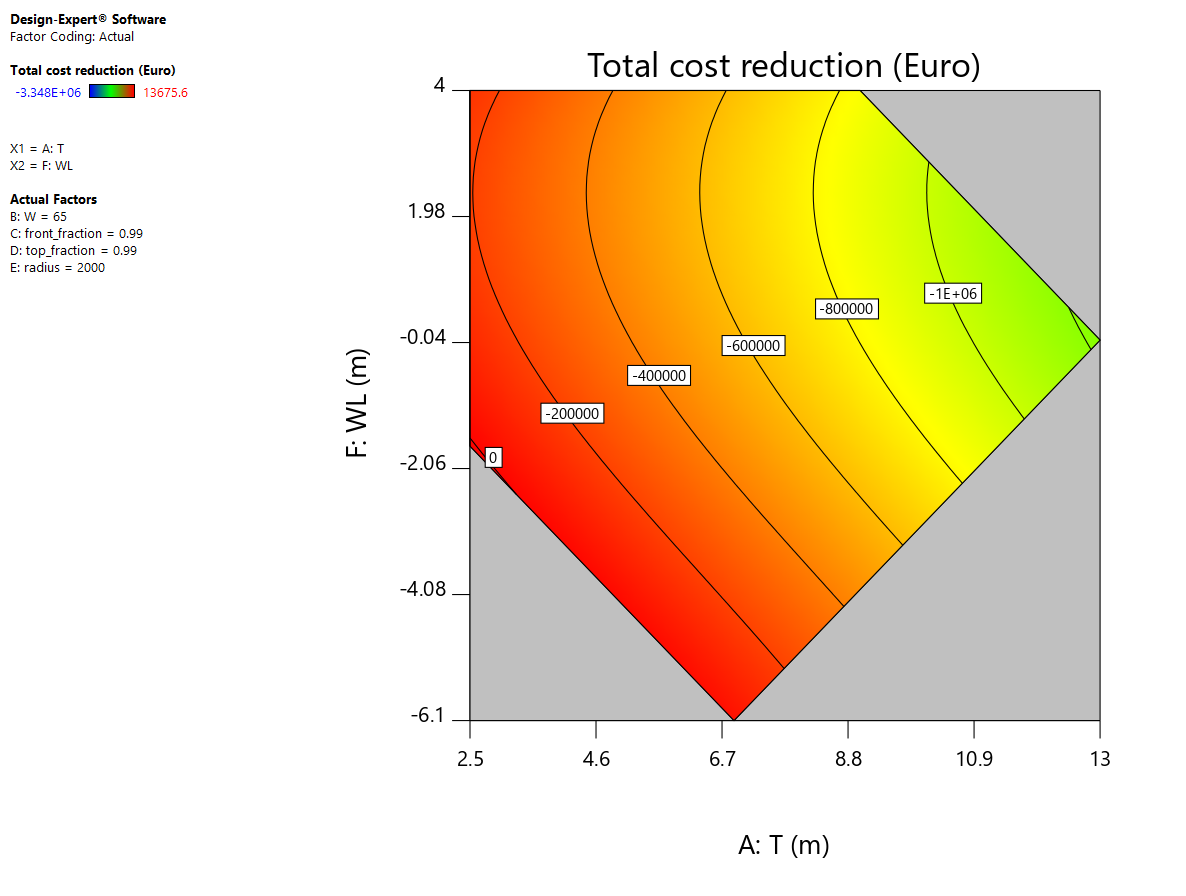
\includegraphics[width=\textwidth]{figures/ComFLOW/Results DI1/costs/T_WL_Costs_total_reduction_box_png.png}
        \caption[]%
        {{\small }}    
        \label{fig: opt }
    \end{subfigure}
    \hfill
    \begin{subfigure}[b]{0.475\textwidth}   
        \centering 
        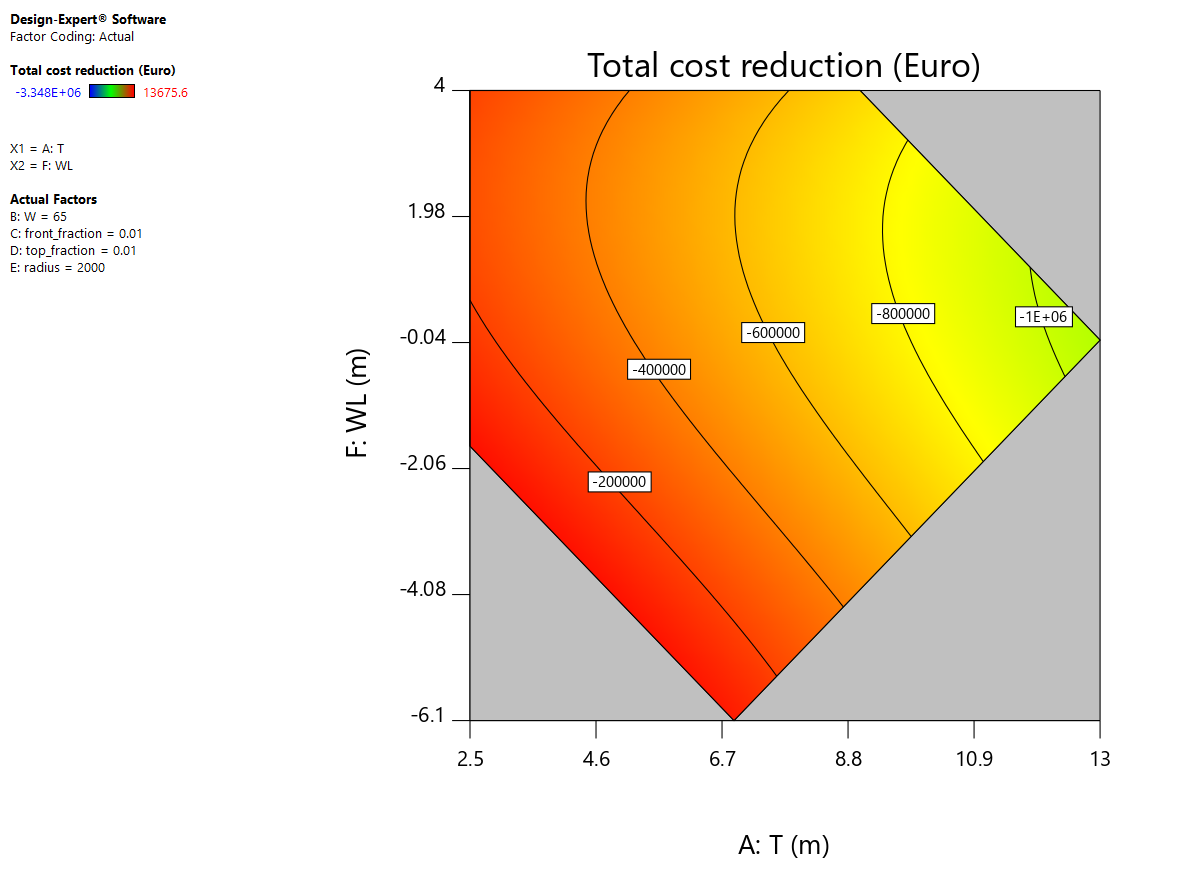
\includegraphics[width=\textwidth]{figures/ComFLOW/Results DI1/costs/T_WL_Costs_total_reduction_wedge_png.png}
        \caption[]%
        {{\small }}    
        \label{fig: opt }
    \end{subfigure}
    \caption{}
    \label{fig: }
\end{figure*}

\begin{figure*}[h]
    \centering
    \begin{subfigure}[b]{0.475\textwidth}   
        \centering 
        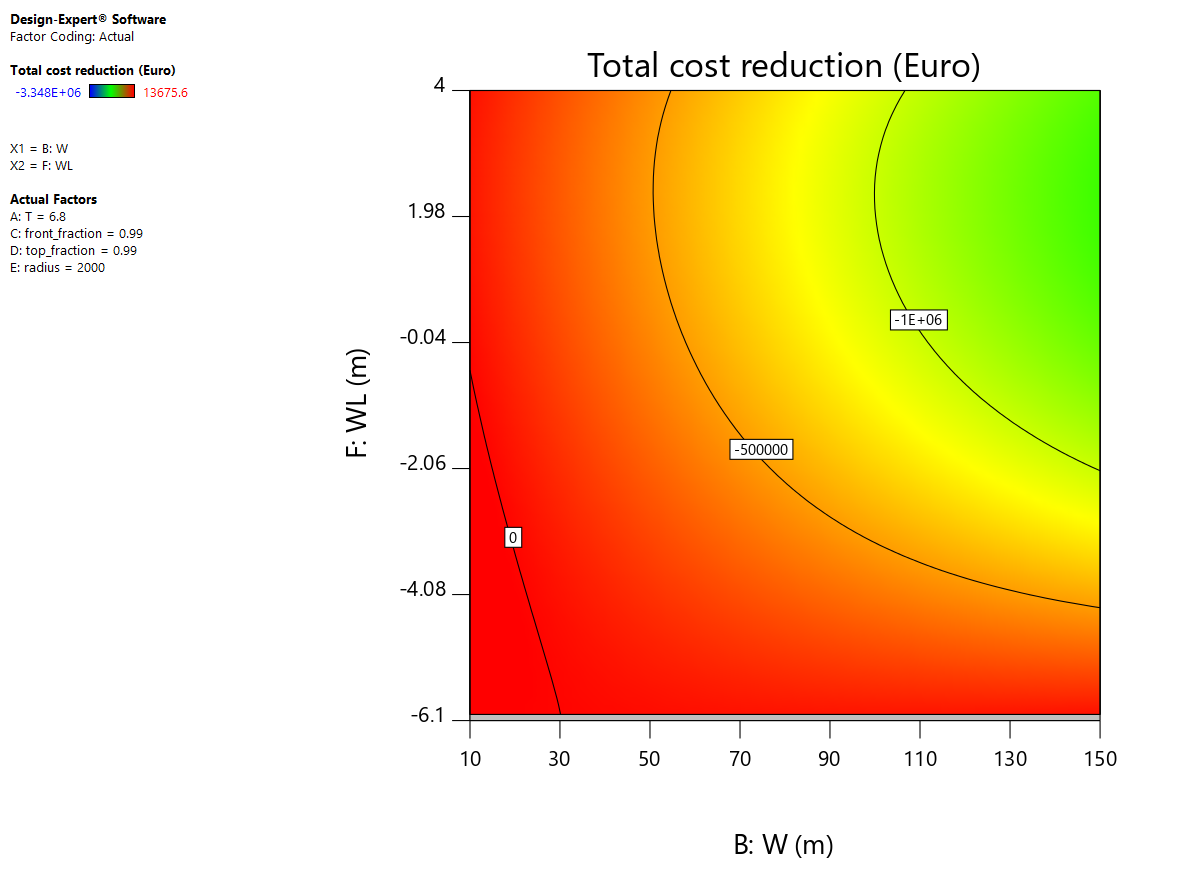
\includegraphics[width=\textwidth]{figures/ComFLOW/Results DI1/costs/W_WL_Costs_total_reduction_box_png.png}
        \caption[]%
        {{\small }}    
        \label{fig: opt }
    \end{subfigure}
    \hfill
    \begin{subfigure}[b]{0.475\textwidth}   
        \centering 
        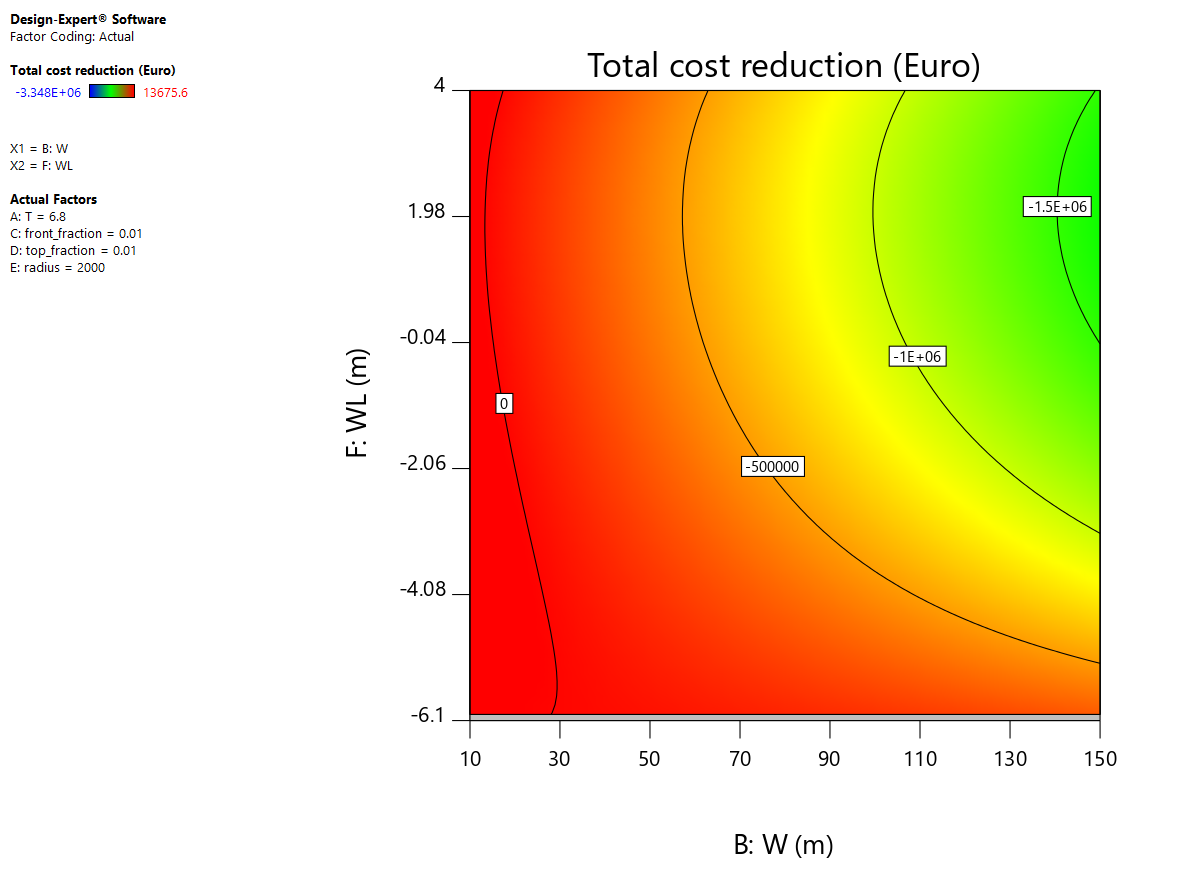
\includegraphics[width=\textwidth]{figures/ComFLOW/Results DI1/costs/W_WL_Costs_total_reduction_wedge_png.png}
        \caption[]%
        {{\small }}    
        \label{fig: opt }
    \end{subfigure}

    \caption{}
    \label{fig: }
\end{figure*}


\begin{table}[H]
\centering
\scalebox{0.65}{
\begin{tabular}{@{}lllllllllllll@{}}
\toprule
configuration & T        & W        & front\_fraction & top\_fraction & radius   & WL & \texteuro$_{total}$ &  \texteuro$_{bw,m}$ & \texteuro$_{new~island}$ & \texteuro$_{reduction}$  & \texteuro$_{bw,c}$  & Desirability   \\ \midrule
1 & 2.50014  & 10.33189 & 0.912045 & 0.99     & 1809.635 & -1.70004  & 158029.9 & 1191.594 & 22912.44 & 25285.3  & -131116  & 0.988171 \\
2 & 2.500945 & 11.67861 & 0.984856 & 0.988659 & 1463.097 & -1.70091  & 150847.1 & 1246.176 & 20894.93 & 26908.7  & -122211  & 0.986146 \\
3 & 2.500224 & 10.53957 & 0.033345 & 0.989996 & 548.1369 & -1.70E+00 & 150606.6 & 191.586  & 15125.16 & 30658.37 & -112472  & 0.986079 \\
4 & 3.227757 & 10.00041 & 0.739436 & 0.989997 & 1997.918 & -2.42758  & 146145.1 & 1547.252 & 24397.77 & 23035.1  & -103263  & 0.984821 \\
5 & 4.294421 & 11.25716 & 0.917247 & 0.989999 & 1999.927 & -3.45615  & 137561.5 & 1743.598 & 28469.58 & 18722.75 & -109104  & 0.982402 \\
6 & 4.15107  & 10.00339 & 0.011256 & 0.98999  & 550.9233 & -3.22E+00 & 136343.8 & 970.0574 & 20016.85 & 26119.13 & -96629.2 & 0.982059  \\ \bottomrule
\end{tabular}
}
\caption{Parameters optimal breakwaters based on  costs}
\label{tab: params design iteration 1 captive 1to6 costs}
\end{table}
where
\begin{itemize}
    \item \texteuro$_{total}$ is the total cost reduction off the mooring system costs
    \item \texteuro$_{bw,m}$ is the height of the costs of the mooring of the breakwater
    \item \texteuro$_{new~island}$ is the height the new mooring cost the island, due to the presence of the breakwater
    \item \texteuro$_{reduction}$ (= \texteuro$_{old~island}$ - \texteuro$_{new~island}$) is the difference between the mooring costs without breakwater and with breakwater.
    \item \texteuro$_{bw,c}$ is the height of the construction costs of the breakwater.
\end{itemize}



\begin{figure*}[h]
    \centering
    \begin{subfigure}[b]{0.475\textwidth}
        \centering
        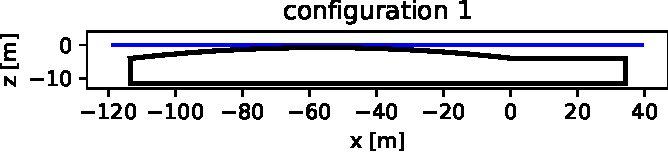
\includegraphics[width=\textwidth]{figures/ComFLOW/Breakwater Geometries/Design Iteration 1 captive/top6 costs/breakwater_geometry1.pdf}
        \caption[]%
        {{\small }}    
        \label{fig: opt }
    \end{subfigure}
    \hfill
    \begin{subfigure}[b]{0.475\textwidth}  
        \centering 
        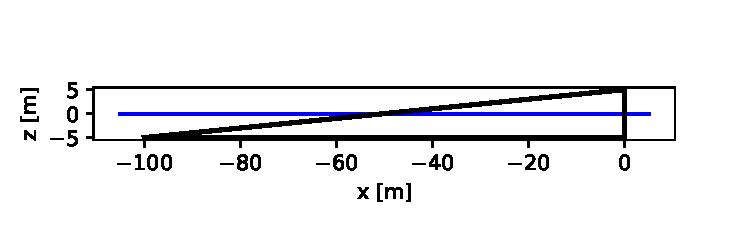
\includegraphics[width=\textwidth]{figures/ComFLOW/Breakwater Geometries/Design Iteration 1 captive/top6 costs/breakwater_geometry2.pdf}
        \caption[]%
        {{\small }}    
        \label{fig: opt }
    \end{subfigure}
    \vskip\baselineskip
    \begin{subfigure}[b]{0.475\textwidth}   
        \centering 
        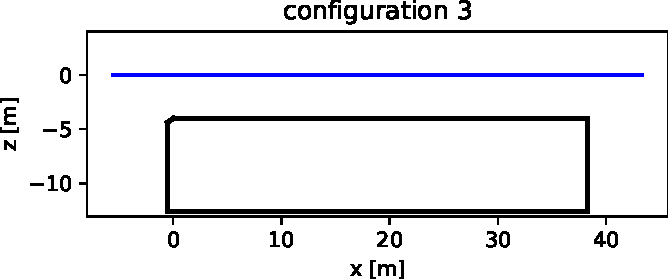
\includegraphics[width=\textwidth]{figures/ComFLOW/Breakwater Geometries/Design Iteration 1 captive/top6 costs/breakwater_geometry3.pdf}
        \caption[]%
        {{\small }}    
        \label{fig: opt }
    \end{subfigure}
    \hfill
    \begin{subfigure}[b]{0.475\textwidth}   
        \centering 
        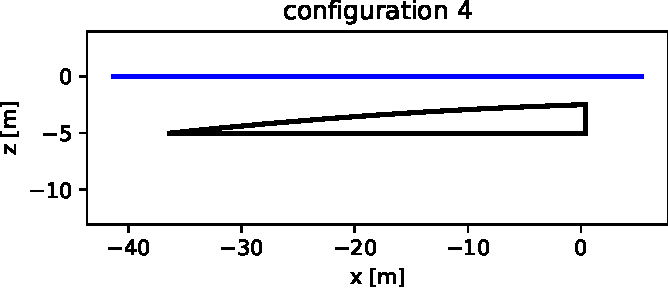
\includegraphics[width=\textwidth]{figures/ComFLOW/Breakwater Geometries/Design Iteration 1 captive/top6 costs/breakwater_geometry4.pdf}
        \caption[]%
        {{\small }}    
        \label{fig: opt }
    \end{subfigure}
    \hfill
    \begin{subfigure}[b]{0.475\textwidth}   
        \centering 
        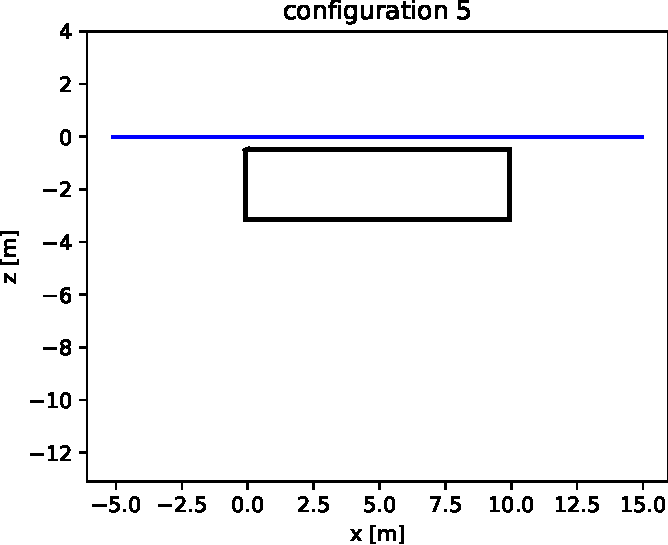
\includegraphics[width=\textwidth]{figures/ComFLOW/Breakwater Geometries/Design Iteration 1 captive/top6 costs/breakwater_geometry5.pdf}
        \caption[]%
        {{\small }}    
        \label{fig: opt }
    \end{subfigure}
        \hfill
    \begin{subfigure}[b]{0.475\textwidth}   
        \centering 
        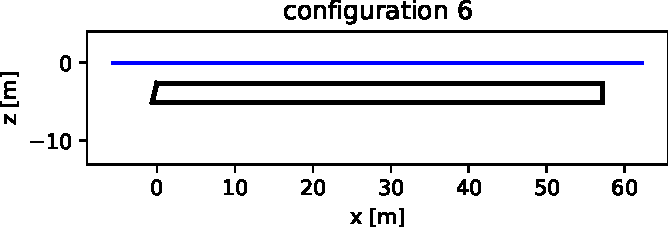
\includegraphics[width=\textwidth]{figures/ComFLOW/Breakwater Geometries/Design Iteration 1 captive/top6 costs/breakwater_geometry6.pdf}
        \caption[]%
        {{\small }}    
        \label{fig: opt }
    \end{subfigure}
    
    \caption{The six most optimal breakwaters based on the reduction in mooring costs}
    \label{fig: six most optimal breakwaters costs}
\end{figure*}



% -mass is used 
% -concrete 775 \texteuro/ton
% -steel 2000-4000 \texteuro/ton 
% (source S@S)
% -steel price depending on how much labour is needed to fabricate. Concrete is not varying, since a varying structure hardly effects the amount of labour, because the concrete is poured in while it is fluid and takes it shape by itself.

% -breakwater divided into two parts, the parts which are rectangular have a price of 2000 \texteuro/ton and the slope has a varying price, depending on the magnitude of the angle shown in this figure:



% \section{Connector costs}
% \label{sec: work and connector costs}



\section{Further costs and benefits}

benefits\\
-workability due to less motions is a major one\\
-more functions of space breakwater: energy generation, growing food (oysters), living, working, storage\\
\\


costs\\
-maintenance breakwaters\\
-hazards of breaking\\
-noise\\




\section{Discussion}

\section{Major assumptions}
-only one component of QTF is indicative of set-up mooring system, back with D3.3 van S@S (tabel 12, load with 1 island module comes is almost the same as my calculation (Note! my calculation is per unit width)\\
-price of mooring system scales linearly with mean wave drift force on system\\
-concrete/steel is used\\
-steel price\\
-concrete price\\
